\documentclass{article}

\usepackage[solutions]{../.template/xrcise}

\subject{Security by Design}
\semester{Winter 2024}
\author{Leopold Lemmermann}

\begin{document}\createtitle

\section{Assignments}

\setcounter{subsection}{10}
\begin{exercise}{Skytala}
  Bei der Skytala handelt es sich um eine Transpositionschiffre, bei der ursprünglich ein Zylinder mit einem Papierstreifen umwickelt wurde. Die Ver- und Entschlüsselung kann aber auch mithilfe einer Matrix dargestellt werden.
  \begin{enumerate}
      \item Verschlüsseln Sie den folgenden Klartext mit einer Skytala, die durch eine Matrix mit sieben Zeilen und neun Spalten beschrieben werden kann:
      \begin{center}
          \texttt{GLUECKLICH\_IST\_DER\_DER\_DEN\_DINGEN\_AUF\_DEN\_GRUND\_GEHEN\_KONNTE}
      \end{center}
      \item Was ist der geheim zu haltende symmetrische Schlüssel der Skytala aus Teilaufgabe a) und wie hängt dieser mit der ursprünglichen Variante mit Zylinder und Papierstreifen zusammen?
      \item Erläutern Sie kurz zwei sinnvolle Ansätze zur Kryptanalyse, d. h. Ansätze zum Brechen einer Skytala.
  \end{enumerate}

  \begin{solution}
    \begin{enumerate}
        \item Verschlüsselung mit Skytala: Teilen Sie den Klartext in eine Matrix mit 7 Zeilen und 9 Spalten:
          \[
          \texttt{GLUECKLICH IST DER DER DEN DINGEN AUF DEN GRUND GEHEN KONNTE}
          \]
          Die Matrix:
          \[
          \begin{array}{ccccccccc}
          G & L & U & E & C & K & L & I & C \\
          H & \_ & I & S & T & \_ & D & E & R \\
          \_ & D & E & R & \_ & D & E & N & \_ \\
          D & I & N & G & E & N & \_ & A & U \\
          F & D & E & N & \_ & G & R & U & N \\
          D & G & E & H & E & N & \_ & K & O \\
          N & T & T & E & \_ & & & & \\
          \end{array}
          \]
          Der Schlüsseltext wird spaltenweise abgelesen: 
          \[
          \texttt{GH\_DDFNLDIRIGTNSEEECEDEINNEK\_CRNUENNUH\_U\_GNGRDKIKAUOE}
          \]
  
        \item Der geheime Schlüssel ist die Größe der Matrix: $ 7 \times 9 $ (Zeilen $\times$ Spalten). Beim ursprünglichen Zylinder entspricht dies dem Umfang des Zylinders.
  
        \item Kryptanalyse:
        \begin{itemize}
            \item Häufigkeitsanalyse: Anhand von Buchstabenhäufigkeiten und Mustererkennung können Transpositionsmuster aufgedeckt werden.
            \item Brute-Force: Alle möglichen Spalten- und Zeilenkombinationen ausprobieren, um den Klartext zu rekonstruieren.
        \end{itemize}
    \end{enumerate}
  \end{solution}
\end{exercise}

\begin{exercise}{Spalten-Transpositionen}
  Bei der Skytala wird ein Zylinder mit einem Papierstreifen umwickelt, beschrieben und wieder abgewickelt.
  \begin{enumerate}
      \item Eine Verbesserung dieser Spalten-Transposition ergibt sich, wenn zusätzlich auch die Spalten in ihrer Reihenfolge vertauscht werden (was beim Papierstreifen natürlich nicht gelingt, wohl aber im Rechner). Um welchen Faktor vergrößert sich dadurch der Schlüsselraum bei $s$ Spalten?
      \item Schreiben Sie eine Skytala mit 4 Zeilen und 3 Spalten (ohne Spaltenvertauschung) in Zyklenschreibweise.
  \end{enumerate}

  \begin{solution}
    \begin{enumerate}
        \item Bei Spaltenvertauschung gibt es $ s! $ mögliche Permutationen für $ s $ Spalten. Der Schlüsselraum vergrößert sich somit um den Faktor $ s! $ im Vergleich zur ursprünglichen Methode ohne Spaltenvertauschung.
  
        \item Klartext in eine $ 4 \times 3 $-Matrix:
          \[
          \texttt{ABCDEFGHIKLMN}
          \]
          In die Matrix eingetragen:
          \[
          \begin{array}{ccc}
          A & B & C \\
          D & E & F \\
          G & H & I \\
          K & L & M \\
          \end{array}
          \]
          Zyklisches Schreiben ergibt:
          \[
          \texttt{ADGKBELHCFIM}
          \]
    \end{enumerate}
  \end{solution}
\end{exercise}

\setcounter{subsection}{20}
\begin{exercise}{Vigenère-Chiffre \ref{ex:vigenere}}\end{exercise}

\begin{exercise}{Zufallszahlen bei der Schlüsselgenerierung}
  Warum sind bei der Schlüsselgenerierung (echte) Zufallszahlen nötig? Weshalb eignet sich die XOR-Verknüpfung, wenn zur Erhöhung der Sicherheit mehrere Zufallszahlen zu einer einzelnen Zufallszahl verknüpft werden, etwa bei der Schlüsselgenerierung?

  \begin{solution}
    \begin{enumerate}
        \item Echte Zufallszahlen sind notwendig, um sicherzustellen, dass Schlüssel nicht vorhersagbar sind. Ein nicht zufälliger Schlüssel kann durch statistische oder deterministische Methoden berechnet werden.
        \item Die XOR-Verknüpfung sichert, dass ein kombinierter Schlüssel nur dann vorhersagbar ist, wenn alle zufälligen Werte vollständig bekannt sind. Dadurch wird ein höherer Grad an Sicherheit erzielt.
    \end{enumerate}
  \end{solution}
\end{exercise}

\begin{exercise}{Falsche Verwendung des One-Time-Pads}
  Ihnen sind eine Reihe verschlüsselter deutscher Substantive in die Hände gefallen. Sie gehen davon aus, dass fahrlässigerweise alle Wörter mit demselben One-Time-Pad verschlüsselt wurden. Versuchen Sie, den Schlüssel zu ermitteln, indem Sie einen geeigneten Angriff implementieren. Die Schlüsseltexte (der 6 Substantive) in Dezimalschreibweise lauten:

  \begin{center}
    \texttt{09 00 04 10} \\
    \texttt{10 20 28 09} \\
    \texttt{10 16 02 02} \\
    \texttt{10 20 05 08} \\
    \texttt{26 26 03 00} \\
    \texttt{28 16 03 17}
  \end{center}

  Hinweis: Das Passwort und die Substantive sind ASCII-codiert (Alphabet = \{A, B, C, ..., Z\}).

  \begin{solution}
    Durch die Wiederverwendung des One-Time-Pads $ k $ für mehrere Nachrichten $ m_1, m_2 $ entsteht folgende Gleichung:
      \[ c_1 \oplus c_2 = (m_1 \oplus k) \oplus (m_2 \oplus k) = m_1 \oplus m_2 \]
    Dies ergibt die XOR-Verknüpfung der Klartexte $ m_1 \oplus m_2 $, die durch Analyse entschlüsselt werden kann. Beispielsweise:
      \[ c_1 = \texttt{09 00 04 10}, \quad c_2 = \texttt{10 20 28 09} \]
    XOR:
      \[ c_1 \oplus c_2 = \texttt{19 20 2C 19} \]
    Häufigkeitsanalysen und bekannte Wörter im Klartext ermöglichen die vollständige Entschlüsselung.
  \end{solution}
\end{exercise}

\begin{exercise}{Grundlagen der Kryptographie}
  \begin{enumerate}
      \item Erläutern Sie zwei Ursachen, die dafür sorgen, dass fast alle kryptographischen Algorithmen mit der Zeit durch andere ersetzt werden müssen.
      \item Sie möchten einen Text so verschlüsseln, dass er auch in 99 Jahren nicht ohne Kenntnis des von Ihnen versteckten Schlüssels entschlüsselt werden kann. Welches Verfahren wählen Sie dazu? Begründen Sie Ihre Entscheidung. Warum wird das Verfahren heutzutage nicht überall benutzt?
      \item In der Vorlesung wurden verschiedene klassische Chiffren behandelt, darunter Substitutionschiffren wie die Caesar-Chiffre (Verschiebechiffre), das Schema von Polybios, das Vigenère-Verfahren und die Vernman-Chiffre. Zudem wurden Transpositionschiffren wie die Skytala betrachtet. Ihnen liegt ein Schlüsseltext vor, der mit einer dieser Chiffren erzeugt wurde. Ihnen ist bekannt, dass es sich um die Verschlüsselung eines deutschen Textes handelt. Wie können Sie – ohne Rechnerunterstützung – vorgehen, um einzugrenzen, welche Chiffre verwendet wurde und erläutern Sie die jeweiligen Ansätze?
  \end{enumerate}

  \begin{solution}
    \begin{enumerate}
        \item Ursachen für Algorithmuswechsel:
        \begin{itemize}
            \item **Technologischer Fortschritt**: Schnellere Computer machen bestimmte Algorithmen unsicher.
            \item **Neue Angriffsmethoden**: Entdeckte Schwachstellen führen zur Ablösung alter Verfahren.
        \end{itemize}
  
        \item Das **One-Time-Pad** bietet langfristige Sicherheit, da es informationstheoretisch sicher ist. Es wird nicht überall genutzt, da Schlüssel so lang wie der Klartext sein müssen und sicher verteilt werden müssen.
  
        \item Bestimmung der Chiffre:
        \begin{itemize}
            \item **Häufigkeitsanalyse**: Substitutionschiffren wie Caesar zeigen typische Muster.
            \item **Permutationsanalyse**: Transpositionen hinterlassen Permutationsmuster.
        \end{itemize}
    \end{enumerate}
  \end{solution}
\end{exercise}

\setcounter{subsection}{30}
\begin{exercise}{Informationstheoretische Sicherheit \ref{ex:otp}}\end{exercise}

\begin{exercise}{Feistel-Prinzip \ref{ex:feistel}}\end{exercise}

\begin{exercise}{Meet-in-the-Middle-Angriff auf 2-DES}
  Um der geringen Schlüssellänge von 56 Bit des DES-Algorithmus zu begegnen, wurde vorgeschlagen, den Algorithmus mehrfach hintereinander mit verschiedenen Schlüsseln anzuwenden. Eine schlechte Lösung ist jedoch die lediglich zweifache Hintereinanderanwendung 2-DES.
  \begin{enumerate}
    \item Vergleichen Sie die Schlüssellänge des 2-DES-Algorithmus mit der tatsächlich erreichten Sicherheit.
    \item Sie haben folgendes Klartext/Schlüsseltext-Paar $ (m, c) $ einer 2-DES-Verschlüsselung $ E_{k_2}(E_{k_1}(m)) = c $ erlangt: 
      \[ m = \texttt{c183 50b5 52b8 f8b1}, \quad c = \texttt{42e0 4462 099e e8ca}. \]
      Ermitteln Sie $ k_1 $ und $ k_2 $, indem Sie einen Meet-in-the-Middle-Angriff durchführen. Benutzen Sie dafür die unten dargestellte Tabelle 1 ausgewählter DES-Funktionswerte. In der Tabelle können für einen gegebenen Klartext $ x $ bzw. einen Schlüsseltext $ y $ und einen Schlüssel $ k $ die Werte der Verschlüsselungsfunktion $ E $ bzw. Entschlüsselungsfunktion $ D $ des DES-Algorithmus nachgeschlagen werden. In welchen Zeilen haben Sie die DES-Funktionswerte, die zum Erfolg beim Meet-in-the-Middle Angriff führen, nachgeschlagen?
      \textit{Hinweis: Beachten Sie das Beispiel zum Ablesen der Tabelle.}
      \begin{table}[H]
  \centering
  \caption{Ausgewählte DES-Funktionswerte}
  \begin{tabular}{c|c|c|c}
  \textbf{Schlüssel $k$} & \textbf{Eingabe $x/y$ von $E_k/D_k$} & \textbf{$E_k(x)$} & \textbf{$D_k(y)$} \\ \hline
  97a4 3741 8086 0b & 6b3b acd4 6570 6187 & fecd 14e2 8cb0 6a2b & 7285 3f6b e44c cb8e \\ \hline
  97a4 3741 8086 0b & 5de1 bd06 54fa 40ed & 42e0 4462 099e e8ca & 9384 bebf 5b18 793f \\ \hline
  3e45 c68f bb89 27 & 5de1 bd06 54fa 40ed & 4995 e68b b800 3a06 & f575 4696 effc 1bf1 \\ \hline
  e6f4 a450 4898 d7 & 764d e3ae 043b d6b7 & 5f31 4917 4ecc e6b4 & 30db 8c29 073a 182c \\ \hline
  f6bb 747d dc16 15 & ceae a65a ae77 1c72 & b1e0 9414 e068 3622 & 9acb 4aff e84a b1f7 \\ \hline
  3e45 c68f bb89 27 & 764d e3ae 043b d6b7 & fca6 8c2f b81e dc79 & 4bae f15e 7efb 5a8c \\ \hline
  e6f4 a450 4898 d7 & c183 50b5 52b8 f8b1 & 5de1 bd06 54fa 40ed & 6b3b acd4 6570 6187 \\ \hline
  3e45 c68f bb89 27 & 9400 39ca 9301 5507 & 199c 2565 ea8e 2b53 & f742 7dac e2ff 00d2 \\ \hline
  f6bb 747d dc16 15 & c620 9b86 c72a 6b3b & 4e6c efc7 1f5b 3756 & 42e0 4462 099e e8ca \\ \hline
  e6f4 a450 4898 d7 & 42e0 4462 099e e8ca & c3fc 30e9 10db 827e & d0eb 0c0e 1b43 12da \\ \hline
  f6bb 747d dc16 15 & a904 aa4e c934 ecb0 & 42e0 4462 099e e8ca & 5617 0d2a ccdb 9981 \\ \hline
  f6bb 747d dc16 15 & a3c5 5b7b c599 e5af & 4179 a965 d79e 1edd & e927 17a5 b2a9 b559 \\ \hline
  e6f4 a450 4898 d7 & 9400 39ca 9301 5507 & 0669 924e 1cec 70d0 & 7555 ce29 f46b 7e74 \\ \hline
  3e45 c68f bb89 27 & 6b3b acd4 6570 6187 & abe6 c175 4435 742a & 043c 252e bbe0 3d09 \\ \hline
  97a4 3741 8086 0b & c183 50b5 52b8 f8b1 & 9400 39ca 9301 5507 & 764d e3ae 043b d6b7 \\ \hline
  97a4 3741 8086 0b & 42e0 4462 099e e8ca & 8b99 c9de 0e47 22db & 5de1 bd06 54fa 40ed \\
  \end{tabular}
\end{table}
    \item Wie viele Einträge enthält eine vollständige Tabelle, die bei einem Meet-in-the-Middle-Angriff auf den 2-DES-Algorithmus erstellt wird, mindestens? Welche Art von Berechnungen werden dort festgehalten?
  \end{enumerate}

  \begin{solution}
    \begin{enumerate}
        \item 2-DES bietet nur $ 2^{56} $ statt $ 2^{112} $ effektiver Sicherheit, da ein Meet-in-the-Middle-Angriff $ E_{k_1}(m) = D_{k_2}(c) $ nutzt.
        \item Analyse aus Tabelle 1:
        \[
        k_1 = \texttt{e6f4 a450 4898 d7}, \quad k_2 = \texttt{97a4 3741 8086 0b}
        \]
        \item Eine vollständige Tabelle umfasst $ 2^{56} $ Einträge, wobei $ E_k(m) $ oder $ D_k(c) $ für alle $ k $ berechnet werden.
    \end{enumerate}
  \end{solution}
\end{exercise}

\begin{exercise}{Triple-DES}
  Beim Triple-DES-Algorithmus (3-DES) handelt es sich um die dreifache Hintereinanderausführung des DES-
  Algorithmus. Dabei wird mit zwei 56 Bit langen Schlüsseln $ k_1 $ und $ k_2 $ gearbeitet und beim Verschlüsseln
  entweder $ E(k_1) \to D(k_2) \to E(k_1) $ (EDE-Modus) oder $ E(k_1) \to E(k_2) \to E(k_1) $ (EEE-Modus) ausgeführt.
  \begin{enumerate}
    \item Warum wird dem EDE-Modus meist der Vorzug vor dem EEE-Modus gegeben?
    \item Berechnen Sie die theoretische und die effektive Schlüssellänge des Triple-DES-Algorithmus unter ei-
    nem Known-Plaintext-Angriff mit drei 56 Bit langen Schlüsseln, d.h. $ E(k_1) \to E(k_2) \to E(k_3) $.
  \end{enumerate}

  \begin{solution}
    \begin{enumerate}
        \item Der EDE-Modus (Encrypt-Decrypt-Encrypt) schützt gegen Meet-in-the-Middle-Angriffe, da die Verschlüsselung durch Entschlüsselung unterbrochen wird.
        \item Die effektive Schlüssellänge beträgt:
        \[
        \text{Theoretisch: } 3 \times 56 = 168 \text{ Bit}, \quad \text{Effektiv: } 112 \text{ Bit (wegen Angriffen).}
        \]
    \end{enumerate}
  \end{solution}
\end{exercise}


\setcounter{subsection}{40}
\begin{exercise}{Unsicherheit des Electronic-Codebook-Modus}
  Eine einfache, jedoch unsichere Technik zum Betrieb einer Blockchiffre ist der Electronic-Codebook-Modus
  (ECB-Modus). Dabei wird jeder Klartextblock unabhängig von den anderen Blöcken chiffriert.
  \begin{enumerate}
    \item Inwiefern stellt dies ein Sicherheitsproblem dar?
    \item Veranschaulichen Sie das Problem, indem Sie ein Programm entwickeln, welches eine einfache Bitmap-Grafik einliest, den Bildinhalt mit dem AES-Verfahren im ECB-Modus verschlüsselt und wieder als Bitmap ausgibt. Rufen Sie zum Vergleich die Verschlüsselung noch einmal im CBC-Modus auf und vergleichen Sie die erhaltenen Resultate. Informieren Sie sich dazu über das Datenformat von BMP-Dateien und die Verwendung einer geeigneten Kryptobibliothek (z. B. die Java-Cryptography-API unter \url{http://www.ibm.com/developerworks/java/tutorials/j-sec1/section4.html} oder die Python-pycrypto- API unter \url{https://www.dlitz.net/software/pycrypto/api/current/}).
  \end{enumerate}

  \begin{solution}
    \begin{enumerate}
        \item Das Hauptproblem des ECB-Modus ist, dass identische Klartextblöcke in identische Schlüsseltextblöcke umgewandelt werden. Dies führt dazu, dass Muster im Klartext auch im Schlüsseltext sichtbar bleiben, was die Sicherheit gefährdet.
        \item Veranschaulichung:
        \begin{itemize}
            \item Entwickeln Sie ein Programm, das eine BMP-Bilddatei einliest und diese im ECB-Modus verschlüsselt. Das resultierende Bild wird die ursprünglichen Muster zeigen, da identische Klartextblöcke identisch verschlüsselt werden.
            \item Im Vergleich dazu führt der CBC-Modus durch die Abhängigkeit jedes Blocks vom vorherigen Block zu einer Verschleierung der Muster.
        \end{itemize}
    \end{enumerate}
  \end{solution}
\end{exercise}

\begin{exercise}{Cipher-Block-Chaining-Betriebsmodus}
  Beim Cipher-Block-Chaining-Betriebsmodus wird ein Klartextblock $ M_i $ vor der Anwendung der Verschlüsselungsfunktion mit dem unmittelbar vorher erzeugten Chiffretextblock $ C_{i-1} $ durch die XOR-Operation verknüpft.
  Die erzeugten Chiffretextblöcke hängen dadurch von ihren Vorgängern ab. Bei der Verschlüsselung des ersten Klartextblocks $ M_1 $ wird für $ C_0 $ ein zufällig gewählter Initialisierungsvektor (IV) verwendet.
  
  Hinweis: Gehen Sie davon aus, dass eine moderne Blockchiffre eingesetzt wird, z. B. AES.
  \begin{enumerate}
    \item Wie unterscheiden sich zwei Schlüsseltexte, die mit demselben Schlüssel erzeugt wurden und denselben Klartext enthalten, jedoch mit unterschiedlichen IVs erzeugt wurden?
    \item Wie unterscheiden sich zwei Schlüsseltexte, wenn sie sich lediglich an einer Stelle im ersten Klartextblock unterscheiden (also ein Bit gekippt wird) und ansonsten völlig identisch sind (bei gleichem IV und Schlüssel)?
    \item Welche Auswirkung hat es beim Entschlüsseln, wenn durch einen Übertragungsfehler ein Bit im zweiten Schlüsseltextblock bei der Übertragung verändert wird?
    \item Welche Auswirkung hat es beim Entschlüsseln, wenn durch einen Übertragungsfehler ein Bit im Initialisierungsvektor verändert wird?
  \end{enumerate}

  \begin{solution}
    \begin{enumerate}
        \item Bei unterschiedlichen IVs führen zwei identische Klartexte zu unterschiedlichen Schlüsseltexten, da der IV die Anfangswerte beeinflusst.
        \item Ein Unterschied in einem Bit im ersten Klartextblock propagiert sich in allen nachfolgenden Schlüsseltextblöcken durch die XOR-Operation.
        \item Ein Fehler im zweiten Schlüsseltextblock wirkt sich nur auf den entsprechenden Klartextblock und den nächsten aus, da der CBC-Modus Block für Block entschlüsselt.
        \item Ein Fehler im IV beeinflusst nur den ersten Klartextblock.
    \end{enumerate}
  \end{solution}
\end{exercise}

\begin{exercise}{Synchronisationsfehler bei Betriebsarten von Blockchiffren}
  Neben additiven Fehlern, bei denen einzelne Bitpositionen oder Nachrichtenabschnitte zufällig oder absichtlich gekippte Bitwerte aufweisen, können auch einzelne Bits oder ganze Blöcke von Nachrichten zufällig oder absichtlich verloren gehen. Wenn etwa ganze Nachrichtenblöcke jeweils einzeln in Datenpaketen transportiert werden, könnte ein verlorenes Datenpaket einen solchen Synchronisationsfehler hervorrufen.
  \begin{enumerate}
    \item Bitte beschreiben Sie die Fehlerfortpflanzung eines Synchronisationsfehlers aufgrund eines verlorenen Nachrichtenblocks beim Electronic Code Book (ECB)-Modus.
    \item Bitte beschreiben Sie die Fehlerfortpflanzung eines Synchronisationsfehlers aufgrund eines verlorenen Bits beim Electronic Code Book (ECB)-Modus.
    \item Wie verhält sich die Fehlerfortpflanzung eines Synchronisationsfehlers beim Cipher Block Chaining (CBC)-Modus, wenn einzelne Bits des übertragenen Ciphertextes verloren gehen?
    \item Bitte vergleichen Sie die Situation einer Fehlerfortpflanzung aufgrund eines Synchronisationsfehlers bei den stromorientierten Betriebsarten mit der bei CBC.
  \end{enumerate}

  \begin{solution}
    \begin{enumerate}
        \item Im ECB-Modus führt der Verlust eines Nachrichtenblocks nicht zu einer Synchronisationsstörung der verbleibenden Blöcke, da jeder Block unabhängig verschlüsselt wird.
        \item Ein verlorenes Bit im ECB-Modus zerstört den betroffenen Block, aber die folgenden Blöcke bleiben lesbar.
        \item Im CBC-Modus führt der Verlust einzelner Bits dazu, dass alle nachfolgenden Blöcke falsch entschlüsselt werden, da der Modus auf den vorherigen Block angewiesen ist.
        \item Bei stromorientierten Betriebsarten (z. B. CTR-Modus) ist die Fehlerfortpflanzung auf den aktuellen Block beschränkt, da kein Feedback aus vorherigen Blöcken verwendet wird. Dies ist ein Vorteil gegenüber CBC.
    \end{enumerate}
  \end{solution}
\end{exercise}

\setcounter{subsection}{50}
\begin{exercise}{Verketteter Cipher-Block-Chaining-Betriebsmodus}
  Beim verketteten Cipher-Block-Chaining-Betriebsmodus wird zur Steigerung des Datendurchsatzes nur für die erste Nachricht $ M_1 $ ein Initialisierungsvektor $ IV $ gewählt. Das heißt für den Schlüsseltext $ C_1 = C_1^0 || \ldots || C_1^{n_1} $ der ersten Nachricht $ M_1 = M_1^1 || \ldots || M_1^{n_1} $ gilt wie beim normalen CBC:
  \[
      C_1^0 = IV, \quad C_1^i = E(C_1^{i-1} \oplus M_1^i, K) \quad \text{mit } i = 1, \ldots, n_1.
  \]
  Für alle folgenden Nachrichten $ M_2, \ldots $ wird anstelle des $ IV $ der letzte Schlüsseltextblock des vorherigen Schlüsseltextes verwendet. Das heißt für den Schlüsseltext $ C^j = C^j_1 || \ldots || C^j_{n_j} $ aller weiteren Nachrichten $ M_j = M_j^1 || \ldots || M_j^{n_j} $ mit $ j > 1 $ gilt:
  \[
      C^j_1 = E(C^{j-1}_{n_{j-1}} \oplus M_j^1, K), \quad C^j_i = E(C^j_{i-1} \oplus M_j^i, K) \quad \text{mit } i = 2, \ldots, n_j.
  \]
  \begin{enumerate}
    \item Berechnen Sie unter Angabe aller Zwischenschritte die prozentuale Erhöhung des Datendurchsatzes. Führen Sie die Berechnungen sowohl für einen Block als auch für vier Blöcke pro Nachricht aus. Gehen Sie in beiden Fällen von insgesamt $ 2^{20} $ zu verschlüsselnden Nachrichten vor Neugenerierung eines Schlüssels und Neustart mit einem neuen $ IV $ aus.
    \item Ihnen ist ein Schlüsseltext $ C^j $ in die Hände gefallen, der nur aus zwei möglichen Klartexten $ M_j $ oder $ \tilde{M}_j $ gebildet worden sein kann. Erläutern Sie, wie Sie ermitteln könnten, welcher der beiden Klartexte verschlüsselt wurde, wenn Sie den Klartext $ M_{j+1} $ für die nächste Nachricht selbst wählen dürfen.
    \item Beschreiben Sie ein Szenario für einen derartigen Angriff.
    \item Bewerten Sie ausgehend von der bisherigen Diskussion die Folge selbst kleinster Änderungen für die Sicherheit kryptographischer Algorithmen.
  \end{enumerate}

  \begin{solution}
    \begin{enumerate}
        \item Bei einem verketteten CBC-Modus steigt der Datendurchsatz, da kein neuer IV benötigt wird. Für $ 2^{20} $ Nachrichten bei einer Blockgröße von $ 128 $ Bit beträgt der Effizienzgewinn ca. 0,01\%, da der Initialisierungsaufwand entfällt.
        \item Wenn $ M_j $ oder $ \tilde{M}_j $ verschlüsselt wurde, kann durch die Manipulation des nächsten Klartextblocks $ M_{j+1} $ festgestellt werden, welcher Klartext verwendet wurde. Dies ermöglicht einen Known-Plaintext-Angriff.
        \item Ein mögliches Szenario: Ein Angreifer, der Zugriff auf den Kommunikationskanal hat, modifiziert gezielt den nächsten Klartextblock, um Rückschlüsse auf vorherige Blöcke zu ziehen.
        \item Selbst kleinste Änderungen im Verfahren können signifikante Sicherheitsrisiken schaffen. Hier: Die Wiederverwendung des letzten Blocks des vorherigen Schlüsseltextes anstelle eines neuen IVs.
    \end{enumerate}
  \end{solution}
\end{exercise}

\begin{exercise}{Indeterministische Verschlüsselung \ref{ex:indeterministic}}\end{exercise}

\begin{exercise}{Elliptische Kurven: Grundlagen}
  Elliptic Curve Cryptography (ECC) bezeichnet asymmetrische Kryptosysteme, die auf Operationen auf elliptischen Kurven über endlichen Körpern aufbauen.
  \begin{enumerate}
    \item Erläutern Sie, auf welchem mathematischen Problem die Sicherheit von ECC beruht.
    \item Beschreiben Sie, wie der Diffie-Hellman-Schlüsselaustausch auf Basis von ECC aussehen könnte.
    \item Welche Vorteile bietet ECC gegenüber Kryptosystemen wie RSA?
  \end{enumerate}

  \begin{solution}
    \begin{enumerate}
        \item Die Sicherheit von ECC beruht auf dem Problem der diskreten Logarithmen über elliptischen Kurven, das als schwer lösbar gilt.
        \item Der Diffie-Hellman-Schlüsselaustausch funktioniert, indem beide Kommunikationspartner Punkte auf der elliptischen Kurve austauschen und einen gemeinsamen Punkt berechnen.
        \item Vorteile von ECC:
        \begin{itemize}
            \item Kürzere Schlüssel bei gleicher Sicherheit (z. B. ECC-256 entspricht RSA-3072).
            \item Geringerer Speicher- und Rechenaufwand.
        \end{itemize}
    \end{enumerate}
  \end{solution}
\end{exercise}

\begin{exercise}{Elliptische Kurven: Rechenbeispiele zur Punktaddition}
  Gegeben sei die elliptische Kurve $E(\mathbb{GF}(p))$ mit $a = 1, b = 6, p = 11$:
    \[ E(\mathbb{GF}(11)) : y^2 \equiv x^3 + x + 6 \pmod{11} \]
  \textit{Hinweis: Wir betrachten für diese Aufgabe die in der Kryptographie häufig genutzten elliptischen Kurven über $ \mathbb{Z}_p $ der Form $f(x, y) : y^2 \equiv x^3 + ax + b \mod p$.}
  \begin{enumerate}
    \item Berechnen Sie die Punkte, die auf dieser Kurve liegen.
    \item Suchen Sie sich zwei beliebige Punkte auf der Kurve und addieren Sie diese. Wie funktioniert die Punktaddition im Allgemeinen?
    \item Berechnen Sie die skalare Multiplikation des Punktes $(2, 4)$ mit dem Skalar $ 3 $. Was ist das allgemeine Vorgehen hier?
  \end{enumerate}

  \begin{solution}
    \begin{enumerate}
        \item $\{(2,4), (2,7), (3,9), (3,2), (5,2), (5,8), (7,5), (7,6), (8,9), (8,2), (10,1), (10,10)\}$
        \item $P+Q=(2,4)+(5,2)=(5,2)$.
          \[
            m=\begin{cases}
              \frac{3x_P^2+a}{2y_P} \quad \text{falls } P=Q \\
              \frac{y_Q-y_P}{x_Q-x_P}
            \end{cases} \quad
            \begin{array}{l}
              x_R=m^2-x_P-x_Q\\
              y_R=m(x_R-x_{P|Q})-y_{P|Q}
            \end{array} \pmod{p} \]
        \item $3 \cdot (2,4)=(2,4)$. Double-and-add:
          \[ nP=2^{k-1}P+2^{k-2}P+\ldots+2P+P \]
    \end{enumerate}
  \end{solution}
\end{exercise}

\setcounter{subsection}{60}
\begin{exercise}{RSA: Eigenschaften und Sicherheit \ref{ex:rsa}}\end{exercise}

\begin{exercise}{Forward Secrecy mit RSA}
  Zur Erreichung von Forward Secrecy erzeugt Alice auf ihrem Server mit dem RSA-Verfahren einen privaten Schlüssel $d$ sowie den dazu passenden öffentlichen Schlüssel $c$, den sie persönlich an ihre Nutzerinnen und Nutzer verteilt. Zusätzlich erzeugt der Server von Alice bei jedem Verbindungsaufbau ein neues kurzlebiges (engl. ephemeral) RSA-Schlüsselpaar, das aus einem öffentlichen Schlüssel $ c_e $ und einem geheimen Schlüssel $ d_e $ besteht. Der Server signiert mit dem privaten Schlüssel $ d $ den neuen öffentlichen Schlüssel $ c_e $ und sendet diesen zusammen mit der Signatur über die aufgebaute Verbindung an die Kundin. Die Kundin prüft anschließend die Signatur mithilfe des zuvor von Alice erhaltenen öffentlichen Schlüssels $ c $.
  \begin{enumerate}
    \item Welche Verbindungen könnten von einem sehr starken Angreifer wie einem Nachrichtendienst noch entschlüsselt werden, wenn dieser an $1$ gelangt? Begründen Sie Ihre Antwort.
    \item Skizzieren Sie einen Angriff, der möglich wäre, wenn die Kundin die Signatur nicht prüft.
    \item Alice ist das Verfahren zu langsam. Sie nimmt folgende Änderung vor: Statt jedes Mal bei der Erzeugung von $c_e$ und $d_e$ neue Primzahlen $p$ und $q$ für den Modulus $N_e$ zu generieren, verwendet sie immer die gleichen Primzahlen. Nun wählt sie lediglich den öffentlichen Exponenten $ c_e $ neu und berechnet einen dazugehörigen geheimen Exponenten $ d_e $. Warum ist dies keine gute Idee? Zeigen Sie, wie sich dieses geänderte Verfahren angreifen lässt, um aufgezeichnete Verbindungen zu entschlüsseln.
  \end{enumerate}

  \begin{solution}
    \begin{enumerate}
      \item Ein starker Angreifer kann alle Verbindungen entschlüsseln, wenn er $d$ erhält, da er damit alle geheimen Schlüssel $d_e$ berechnen kann.
      \item Es könnten gefälschte öffentliche Schlüssel $c_e$ und Signaturen an die Kundin gesendet werden, die nicht von Alice stammen.
      \item Durch die Verwendung der gleichen Primzahlen $p$ und $q$ für $N$ und $N_e$ kann ein Angreifer $d$ berechnen, wenn er $d_e$ kennt. Dies ermöglicht das Entschlüsseln aller Verbindungen.
    \end{enumerate}
  \end{solution}
\end{exercise}

\begin{exercise}{Diffie-Hellman-Schlüsselaustauschprotokoll}
  Das Diffie-Hellman-Schlüsselaustauschprotokoll (DH-Protokoll) ermöglicht es zwei Kommunikationspartnern, durch den Austausch von Nachrichten über einen unsicheren Kanal einen symmetrischen Sitzungsschlüssel zu etablieren, der von passiven Angreifern nicht ermittelt werden kann. Beim ursprünglichen DH-Protokoll, das auch als "anonymes" DH-Protokoll bezeichnet wird, wird kein Schlüsselserver verwendet. Die Kommunikationspartner tauschen dabei erst im Moment des Schlüsselaustausches sämtliche Protokollnachrichten über den unsicheren Kanal aus.
  \begin{enumerate}
    \item Stellen Sie den Ablauf des anonymen DH-Protokolls zwischen den beiden Teilnehmern Alice und Bob mit passend gewählten kleinen Zahlen dar.
    \item Erläutern Sie, auf welcher mathematischen Annahme die Sicherheit des DH-Protokolls basiert. Welche weiteren Annahmen macht man über den Angreifer (Angreifermodell)?
    \item Schutz vor aktiven Angriffen ist möglich, wenn die Kommunikationspartner einige Parameter bzw. Protokollnachrichten vorab über einen sicheren Kanal ausgetauscht haben, der vom Angreifer nicht kontrolliert werden kann. Welche Nachrichten müssen vorab ausgetauscht worden sein, damit aktive Angriffe bemerkt werden können?
  \end{enumerate}

  \begin{solution}
    \begin{enumerate}
        \item $g=5, p=11, \underbrace{a=2, b=3}_\text{geheim}$.\\
          Öffentliche Schlüssel: $\begin{array}{l}
              A\equiv g^a \equiv 5^2 \equiv 3\\
              B\equiv g^b \equiv 5^3 \equiv 4
            \end{array} \pmod{11}$\\
          Gemeinsamer Schlüssel: $K\equiv B^a\equiv A^b\equiv 4^2\equiv 3^3\equiv 5 \pmod{11}$
        \item Sicherheit basiert auf dem diskreten Logarithmusproblem (DLP). Der Angreifer kann $ g^a $ und $ g^b $ nicht effizient in $ a $ und $ b $ umwandeln.
        \item Schutz vor aktiven Angriffen: Vorab-Austausch von $ g, p $ und Authentifizierung der öffentlichen Schlüssel (z. B. durch Signaturen).
    \end{enumerate}
  \end{solution}
\end{exercise}

\begin{exercise}{Elliptische Kurven: EC-ElGamal \ref{ex:elliptic}}\end{exercise}

% \setcounter{subsection}{70}
% \begin{exercise}{}
%  % TODO
%
%   \begin{solution}
%     % TODO
%   \end{solution}
% \end{exercise}

% \setcounter{subsection}{80}
% \begin{exercise}{}
%  % TODO
%
%   \begin{solution}
%     % TODO
%   \end{solution}
% \end{exercise}

% \setcounter{subsection}{90}
% \begin{exercise}{}
%  % TODO
%
%   \begin{solution}
%     % TODO
%   \end{solution}
% \end{exercise}

% \setcounter{subsection}{100}
% \begin{exercise}{}
%  % TODO
%
%   \begin{solution}
%     % TODO
%   \end{solution}
% \end{exercise}

% \setcounter{subsection}{110}
% \begin{exercise}{}
%  % TODO
%
%   \begin{solution}
%     % TODO
%   \end{solution}
% \end{exercise}



\section{Catalogue}

\setcounter{subsection}{46}
\begin{exercise}{Spoofing}
  \begin{enumerate}
    \item Inwiefern kann ein DNS-Spoofing-Angriff für einen Distributed Denial of Service (DDoS)-Angriff ausgenutzt werden? Erklären Sie anschaulich.
    \item Welchen Angriff kann man in der nachfolgenden Ausgabe erkennen? Begründen Sie.
      \begin{center}
        \texttt{?(192.168.1.7) at 00:1f:88:13:fe:f1 [ether] on eth0} \\
        \texttt{?(192.168.1.4) at 00:1f:88:13:fe:f1 [ether] on eth0} \\
        \texttt{?(192.168.1.1) at 00:1f:88:13:fe:f1 [ether] on eth0} \\
        \texttt{?(192.168.1.3) at 00:1f:88:13:fe:f1 [ether] on eth0} \\
        \texttt{?(192.168.1.2) at 00:1f:88:13:fe:f1 [ether] on eth0}
      \end{center}
    \item Warum funktioniert ARP-Spoofing nur in einem lokalen Netz?
    \item Sie vermuten, Opfer eines ARP-Spoofing-Angriffs zu sein. Was können Sie an Ihrem Rechner überprüfen, um einen solchen Angriff erkennen zu können?
  \end{enumerate}

  \begin{solution}
    \begin{enumerate}
        \item Ein DNS-Spoofing-Angriff kann für einen Distributed Denial of Service (DDoS)-Angriff ausgenutzt werden, indem der Angreifer gefälschte DNS-Antworten an Opfer sendet, die zu einem falschen Server führen. Der Server wird durch die massiven Anfragen überlastet.
        \item Die Ausgabe zeigt ein ARP-Spoofing-Angriff. Alle IP-Adressen im lokalen Netzwerk werden mit derselben MAC-Adresse verknüpft (\texttt{00:1f:88:13:fe:f1}). Dadurch kann der Angreifer die Kommunikation zwischen den Teilnehmern überwachen oder manipulieren.
        \item ARP-Spoofing funktioniert nur in lokalen Netzwerken, da ARP (Address Resolution Protocol) nicht über Router hinaus funktioniert. Es ist auf das LAN beschränkt.
        \item Um ARP-Spoofing zu erkennen, können Sie prüfen:
        \begin{itemize}
            \item Stimmen die MAC-Adressen in der ARP-Tabelle mit den bekannten Geräten überein?
            \item Gibt es doppelte Einträge für unterschiedliche IP-Adressen mit derselben MAC-Adresse?
        \end{itemize}
    \end{enumerate}
  \end{solution}
\end{exercise}

\begin{exercise}{Kommunikationsmanipulation}
  Eve und Bob sind befreundet und wohnen im selben Haushalt. Ihre Computer sind an denselben Switch angeschlossen und über diesen mit dem Internet verbunden. Eve hat bald Geburtstag und vermutet, dass Bob ein Geschenk für Sie bei einem Onlineshop bestellen wird, der keine Verbindungsverschlüsselung einsetzt. Einerseits ist sie sehr neugierig und möchte gern so früh wie möglich erfahren, was sie geschenkt bekommt. Andererseits befürchtet sie, dass Bob ihr einen Stoffteddy schenken möchte, den sie nicht haben will. Sie möchte daher Bobs Kommunikation abhören und, wenn nötig, seine Bestellung manipulieren können.
  \begin{enumerate}
    \item\label{itm:manipulation} Nennen und erläutern Sie eine Angriffsart, mit der Eve den gesamten Netzverkehr von Bob abhören und manipulieren kann.
    \item Wie kann Bob sich vor dem in Teilaufgabe \ref{itm:manipulation} beschriebenen Angriff schützen?
  \end{enumerate}

  \begin{solution}
    \begin{enumerate}
        \item Eve kann einen \textbf{Man-in-the-Middle-Angriff (MITM)} durchführen, indem sie ARP-Spoofing einsetzt. Sie fälscht die Zuordnung der IP-Adressen zu MAC-Adressen, sodass der gesamte Netzverkehr von Bob über ihren Computer geleitet wird. Eve kann die Daten lesen und manipulieren.
        \item Bob kann sich schützen durch:
        \begin{itemize}
            \item Nutzung von HTTPS für verschlüsselte Verbindungen.
            \item Aktivieren von ARP-Schutzmechanismen (z. B. ARP-Wächter).
            \item Überprüfung von SSL-Zertifikaten auf Authentizität.
        \end{itemize}
    \end{enumerate}
  \end{solution}
\end{exercise}

\setcounter{subsection}{104}
\begin{exercise}{Indeterministische Verschlüsselung}\label{ex:indeterministic}
  \begin{enumerate}
    \item Was bedeutet indeterministische Verschlüsselung?
    \item\label{itm:asymmetric} Wie realisieren Sie die indeterministische Verschlüsselung bei einem asymmetrischen Konzelationssystem?
    \item Was ändert sich gegenüber \ref{itm:asymmetric} bei einem symmetrischen Konzelationssystem?
    \item Sie sollen eine indeterministische Verschlüsselung realisieren. Zur Auswahl stehen die Algorithmen RSA und ElGamal. Wie würden Sie bei beiden Algorithmen vorgehen?
    \item Beim Einsatz asymmetrischer Verschlüsselung sollte eine Nachricht vor der Verschlüsselung noch um (Pseudo-)Zufallszahlen ergänzt werden (indeterministische Verschlüsselung). Welcher Angriff kann dadurch verhindert werden?
  \end{enumerate}

  \begin{solution}
    \begin{enumerate}
        \item Indeterministische Verschlüsselung bedeutet, dass derselbe Klartext bei wiederholter Verschlüsselung mit demselben Schlüssel unterschiedliche Schlüsseltexte erzeugt.
        \item Bei einem asymmetrischen Verschlüsselungssystem kann indeterministische Verschlüsselung durch die Einbeziehung eines Zufallswerts (zB. Padding mit Zufallszahlen) in die Nachricht erreicht werden.
        \item Bei einem symmetrischen Verschlüsselungssystem kann dies durch die Verwendung eines Initialisierungsvektors (IV) realisiert werden.
        \item Verfahren:
        \begin{itemize}
            \item **RSA**: Fügen Sie der Nachricht einen zufälligen Wert hinzu (z. B. OAEP-Padding).
            \item **ElGamal**: Verwenden Sie bei jeder Verschlüsselung einen neuen Zufallswert.
        \end{itemize}
        \item Indeterministische Verschlüsselung verhindert einen **Known-Plaintext-Angriff**, bei dem der Angreifer durch die Analyse von wiederholt verschlüsselten Nachrichten auf den Klartext schließen könnte.
    \end{enumerate}
  \end{solution}
\end{exercise}

\begin{exercise}{Informationstheoretische Sicherheit}\label{ex:otp}
  Das One-Time-Pad (Vernam-Chiffre) ist ein sehr einfaches, aber informationstheoretisch sicheres symmetrisches Verschlüsselungsverfahren: Die Klartextbits $x_i$ werden einzeln XOR-verknüpft mit einer zufälligen Schlüsselfolge $k_i$ gleicher Länge, die nur ein einziges Mal verwendet werden darf (Schlüsseltext $s_i = x_i \oplus k_i$ mit $i= 1,2,...$).
  \begin{enumerate}
    \item Was erfährt der Angreifer, der den Schlüsseltext abfängt, über den Klartext?
    \item Wie würden Sie die Sicherheit des Verfahrens beweisen?
    \item Warum darf die Schlüsselfolge nicht mehrmals verwendet werden? Überlegen Sie sich, was passieren würde, wenn der Angreifer zwei Schlüsseltexte $s_1$ und $s_2$ (oder gar noch weitere) abfangen würde, die unter dem gleichen Schlüssel $k= k_1 = k_2$ verschlüsselt wurden (Annahme: Es handelt sich um sinnvolle Klartexte).
    \item Es existiert auch ein informationstheoretisch sicheres (symmetrisches) Verfahren zur Authentifikation. Welche Eigenschaft muss ein informationstheoretisch sicheres Authentifikationssystem besitzen?
    \item Entwerfen Sie ein solches System und erläutern Sie dessen Funktionsweise sowie dessen Schutz vor einem Angreifer und damit dessen informationstheoretische Sicherheit. Legen Sie eine bitweise Authentisierung (ein MAC-Bit pro Klartextbit) zugrunde.
    \item Kann es informationstheoretisch sichere asymmetrische Verfahren zur Verschlüsselung bzw. Authentifikation geben? Begründen Sie Ihre Antwort.
  \end{enumerate}

  \begin{solution}
    \begin{enumerate}
        \item Lediglich die Länge des Klartexts. Der Klartext bleibt geheim.
        \item Sicherheit des Verfahrens: $H(M|C) = H(M)$ (Entropie bleibt erhalten). Der Schlüsseltext enthält keine Informationen über den Klartext ohne den Schlüssel.
        \item Wiederverwendung des Schlüssels: $C_1 \oplus C_2 = M_1 \oplus M_2$. Dies ermöglicht die Rekonstruktion der Klartexte $M_1, M_2$.
        \item Ein informationstheoretisch sicheres Authentifikationssystem muss auf zufälligen, einmaligen Schlüsseln basieren (z. B. MACs mit OTPs).
        \item Schlüssel und Hashfunktion austauschen. Sender: MAC erstellen $t_i=h(k_i, m_i)$. Empfänger: MAC überprüfen $t_i=h(k_i, m'_i)$.
        \item Es gibt keine informationstheoretisch sicheren asymmetrischen Verfahren, da der öffentliche Schlüssel immer Angriffsvektoren bietet.
    \end{enumerate}
  \end{solution}
\end{exercise}

\setcounter{subsection}{112}
\begin{exercise}{Unsicherheit der klassischen Verschiebechiffre}\label{ex:vigenere}
  Ein klassisches Verschlüsselungsverfahren ist die Verschiebechiffre (Vigenère-Chiffre). Sie arbeitet typischerweise auf einem Alphabet aus den Großbuchstaben A-Z für den Klartext, den Schlüssel und den Schlüsseltext. Zudem kann ein Zeichen zur Worttrennung hinzugenommen werden. Für diese Aufgabe wird dazu der Unterstrich \texttt{\_} verwendet. Ein Schlüsseltextzeichen ergibt sich aus dem um das Schlüsselzeichen verschobene Klartextzeichen. Dieses sogenannte Vigenère-Tableau ist in Abbildung 1 dargestellt.
  \begin{table}[H]
  \center
  \setlength{\tabcolsep}{1pt}
  \begin{tabular}{c|ccccc ccccc ccccc ccccc ccccc cc}
    & A & B & C & D & E & F & G & H & I & J & K & L & M & N & O & P & Q & R & S & T & U & V & W & X & Y & Z & \_ \\
    \hline
    A & A & B & C & D & E & F & G & H & I & J & K & L & M & N & O & P & Q & R & S & T & U & V & W & X & Y & Z & \_ \\
    B & B & C & D & E & F & G & H & I & J & K & L & M & N & O & P & Q & R & S & T & U & V & W & X & Y & Z & \_ & A \\
    C & C & D & E & F & G & H & I & J & K & L & M & N & O & P & Q & R & S & T & U & V & W & X & Y & Z & \_ & A & B \\
    D & D & E & F & G & H & I & J & K & L & M & N & O & P & Q & R & S & T & U & V & W & X & Y & Z & \_ & A & B & C \\
    E & E & F & G & H & I & J & K & L & M & N & O & P & Q & R & S & T & U & V & W & X & Y & Z & \_ & A & B & C & D \\
    F & F & G & H & I & J & K & L & M & N & O & P & Q & R & S & T & U & V & W & X & Y & Z & \_ & A & B & C & D & E \\
    G & G & H & I & J & K & L & M & N & O & P & Q & R & S & T & U & V & W & X & Y & Z & \_ & A & B & C & D & E & F \\
    H & H & I & J & K & L & M & N & O & P & Q & R & S & T & U & V & W & X & Y & Z & \_ & A & B & C & D & E & F & G \\
    I & I & J & K & L & M & N & O & P & Q & R & S & T & U & V & W & X & Y & Z & \_ & A & B & C & D & E & F & G & H \\
    J & J & K & L & M & N & O & P & Q & R & S & T & U & V & W & X & Y & Z & \_ & A & B & C & D & E & F & G & H & I \\
    K & K & L & M & N & O & P & Q & R & S & T & U & V & W & X & Y & Z & \_ & A & B & C & D & E & F & G & H & I & J \\
    L & L & M & N & O & P & Q & R & S & T & U & V & W & X & Y & Z & \_ & A & B & C & D & E & F & G & H & I & J & K \\
    M & M & N & O & P & Q & R & S & T & U & V & W & X & Y & Z & \_ & A & B & C & D & E & F & G & H & I & J & K & L \\
    N & N & O & P & Q & R & S & T & U & V & W & X & Y & Z & \_ & A & B & C & D & E & F & G & H & I & J & K & L & M \\
    O & O & P & Q & R & S & T & U & V & W & X & Y & Z & \_ & A & B & C & D & E & F & G & H & I & J & K & L & M & N \\
    P & P & Q & R & S & T & U & V & W & X & Y & Z & \_ & A & B & C & D & E & F & G & H & I & J & K & L & M & N & O \\
    Q & Q & R & S & T & U & V & W & X & Y & Z & \_ & A & B & C & D & E & F & G & H & I & J & K & L & M & N & O & P \\
    R & R & S & T & U & V & W & X & Y & Z & \_ & A & B & C & D & E & F & G & H & I & J & K & L & M & N & O & P & Q \\
    S & S & T & U & V & W & X & Y & Z & \_ & A & B & C & D & E & F & G & H & I & J & K & L & M & N & O & P & Q & R \\
    T & T & U & V & W & X & Y & Z & \_ & A & B & C & D & E & F & G & H & I & J & K & L & M & N & O & P & Q & R & S \\
    U & U & V & W & X & Y & Z & \_ & A & B & C & D & E & F & G & H & I & J & K & L & M & N & O & P & Q & R & S & T \\
    V & V & W & X & Y & Z & \_ & A & B & C & D & E & F & G & H & I & J & K & L & M & N & O & P & Q & R & S & T & U \\
    W & W & X & Y & Z & \_ & A & B & C & D & E & F & G & H & I & J & K & L & M & N & O & P & Q & R & S & T & U & V \\
    X & X & Y & Z & \_ & A & B & C & D & E & F & G & H & I & J & K & L & M & N & O & P & Q & R & S & T & U & V & W \\
    Y & Y & Z & \_ & A & B & C & D & E & F & G & H & I & J & K & L & M & N & O & P & Q & R & S & T & U & V & W & X \\
    Z & Z & \_ & A & B & C & D & E & F & G & H & I & J & K & L & M & N & O & P & Q & R & S & T & U & V & W & X & Y \\
    \_ & \_ & A & B & C & D & E & F & G & H & I & J & K & L & M & N & O & P & Q & R & S & T & U & V & W & X & Y & Z
  \end{tabular}
  
  \caption{Vigenère-Tableau}
  \label{tbl:vigenere}
\end{table}

% TODO: add table
  % A B C D E F G H I J K L M N O P Q R S T U V W X Y Z _
  %
  % A A B C D E F G H I J K L M N O P Q R S T U V W X Y Z _
  % B B C D E F G H I J K L M N O P Q R S T U V W X Y Z _ A
  % C C D E F G H I J K L M N O P Q R S T U V W X Y Z _ A B
  % D D E F G H I J K L M N O P Q R S T U V W X Y Z _ A B C
  % E E F G H I J K L M N O P Q R S T U V W X Y Z _ A B C D
  % F F G H I J K L M N O P Q R S T U V W X Y Z _ A B C D E
  % G G H I J K L M N O P Q R S T U V W X Y Z _ A B C D E F
  % H H I J K L M N O P Q R S T U V W X Y Z _ A B C D E F G
  % I I J K L M N O P Q R S T U V W X Y Z _ A B C D E F G H
  % J J K L M N O P Q R S T U V W X Y Z _ A B C D E F G H I
  % K K L M N O P Q R S T U V W X Y Z _ A B C D E F G H I J
  % L L M N O P Q R S T U V W X Y Z _ A B C D E F G H I J K
  % M M N O P Q R S T U V W X Y Z _ A B C D E F G H I J K L
  % N N O P Q R S T U V W X Y Z _ A B C D E F G H I J K L M
  % O O P Q R S T U V W X Y Z _ A B C D E F G H I J K L M N
  % P P Q R S T U V W X Y Z _ A B C D E F G H I J K L M N O
  % Q Q R S T U V W X Y Z _ A B C D E F G H I J K L M N O P
  % R R S T U V W X Y Z _ A B C D E F G H I J K L M N O P Q
  % S S T U V W X Y Z _ A B C D E F G H I J K L M N O P Q R
  % T T U V W X Y Z _ A B C D E F G H I J K L M N O P Q R S
  % U U V W X Y Z _ A B C D E F G H I J K L M N O P Q R S T
  % V V W X Y Z _ A B C D E F G H I J K L M N O P Q R S T U
  % W W X Y Z _ A B C D E F G H I J K L M N O P Q R S T U V
  % X X Y Z _ A B C D E F G H I J K L M N O P Q R S T U V W
  % Y Y Z _ A B C D E F G H I J K L M N O P Q R S T U V W X
  % Z Z _ A B C D E F G H I J K L M N O P Q R S T U V W X Y
  % _ _ A B C D E F G H I J K L M N O P Q R S T U V W X Y Z
  % Abbildung 1: Vigenère-Tableau
  \begin{enumerate}
    \item Verschlüsseln Sie den nachfolgenden Klartext mit dem Schlüsselwort PRUEFUNG unter Verwendung einer Vigenère-Chiffre:
    \begin{center}
        \texttt{GLUECKLICH\_IST\_DER\_DER\_DEN\_DINGEN\_AUF\_DEN\_GRUND\_GEHEN\_KONNTE}
    \end{center}
    \item Erläutern Sie kurz zwei sinnvolle Ansätze zur Kryptanalyse, d. h. zum Brechen einer Vigenère-Chiffre.
    \item Eine Verbesserung der Vigenère-Chiffre ergibt sich durch die Verlängerung des Schlüsselwortes. Um welchen Faktor vergrößert sich dadurch der Schlüsselraum bei einem Alphabet mit 27 Elementen (A-Z und Unterstrich als Worttrennung) und einer Verlängerung um $s$ Zeichen?
    \item Wie müsste die Vigenère-Chiffre verändert werden, um informationstheoretische Sicherheit im Bezug auf die Vertraulichkeit zu liefern? Begründen Sie, warum dieser Veränderung zielführend ist.
  \end{enumerate}

  \begin{solution}
    \begin{enumerate}
        \item Verschlüsselung mit PRUEFUNG als Schlüssel: $C = \texttt{ILNUHAZKA\_VLA\_ANL\_KLU\_LTS\_GMMI\_VQK\_TVT\_OZUB\_DRNT\_OZXEU}$
        \item Kryptanalyse:
          \begin{itemize}
              \item Häufigkeitsanalyse, um Muster aufzudecken.
              \item Analyse von Periodizitäten, um die Schlüssellänge zu bestimmen.
          \end{itemize}
        \item Verlängerung des Schlüsselworts: $\text{Faktor der Vergrößerung: } 27^s$
        \item Um informationstheoretische Sicherheit zu erreichen, müsste das Verfahren in ein One-Time-Pad umgewandelt werden. Dazu müsste der Schlüssel genauso lang wie der Klartext und zufällig sein.
    \end{enumerate}
  \end{solution}
\end{exercise}

\begin{exercise}{Klassische Chiffren und Gütekriterien}
  \begin{enumerate}
    \item Verschlüsseln Sie den Klartext PRUEFUNGSSPASS\_OHNE\_KOMPROMISSE mit der Skytala und dem Schlüssel $k= 4$ (4 Zeilen, 8 Spalten). Verschlüsseln Sie den Klartext STUDIUMSFREUDE mit der Caesar-Chiffre und dem Schlüssel $k= 3$.
    \item Die sogenannte Häufigkeitsanalyse kann als Angriff auf klassische Chiffren verwendet werden. Dabei werden die Buchstabenhäufigkeiten eines Chiffretextes gezählt und mit den normalerweise vorkommenden Buchstabenhäufigkeiten von Klartexten verglichen. Damit können Rückschlüsse von den Chiffretextbuchstaben auf die Klartextbuchstaben gezogen werden. Für welche der beiden in Teilaufgabe a) angesprochenen klassischen Chiffren ist dieser Angriff besonders schwerwiegend und kann zum direkten Brechen einer Chiffre führen? Begründen Sie Ihre Antwort.
    \item Sie kommen auf die Idee, beide Chiffren miteinander zu kombinieren, um eine größere Sicherheit zu erreichen. Begründen Sie für die Variante, dass zuerst die Caesar-Chiffre auf den Klartext und dann die Skytala auf den resultierenden Caesar-Chiffretext angewandt wird, ob diese Überlegung tatsächlich stimmt. Ändert sich an Ihrer Überlegung etwas, wenn erst die Skytala und dann die Caesar-Chiffre angewandt wird?
    \item Nennen und erläutern Sie die Gütekriterien, die moderne symmetrische Chiffren erfüllen müssen, um vor derartig einfachen Angriffen wie der Häufigkeitsanalyse zu schützen.
  \end{enumerate}

  \begin{solution}
    \begin{enumerate}
        \item Verschlüsselung:
        \begin{itemize}
            \item Mit der Skytala ($k = 4$): $\texttt{PRUEFUNGSSPASS\_OHNE\_KOMPROMISSE} \rightarrow \texttt{PSHRRSNOUPEMEA\_IFSKSUSOSN\_MEGOP}$
            \item Mit der Caesar-Chiffre ($k = 3$): $\texttt{STUDIUMSFREUDE} \rightarrow \texttt{VWXGLXPVIKUHGH}$
        \end{itemize}
        \item Häufigkeitsanalyse:
          \begin{itemize}
              \item Besonders problematisch bei der Caesar-Chiffre, da Buchstabenhäufigkeiten direkt übertragen werden.
              \item Die Skytala bewahrt Buchstabenhäufigkeiten ebenfalls, ist jedoch schwieriger zu entschlüsseln, da Permutationen involviert sind.
          \end{itemize}
        \item Da beide Chiffren unabhängig voneinander angewendet werden und individuell schwach sind, ist die Sicherheit nicht stark erhöht. Reihenfolge der Anwendung ist irrelevant, da beide Operationen kommutativ sind.
        \item Moderne Chiffren müssen folgende Gütekriterien erfüllen:
          \begin{itemize}
              \item \textbf{Konfusionsanforderung}: Beziehung zwischen Klartext und Schlüsseltext sollte möglichst komplex sein.
              \item \textbf{Diffusionsanforderung}: Änderungen eines Klartextbits sollten viele Schlüsseltextbits beeinflussen.
              \item \textbf{Resistenz gegen Kryptoanalyse}: Gegenüber modernen Angriffen wie Brute-Force, statistischen und algebraischen Angriffen sicher.
          \end{itemize}
    \end{enumerate}
  \end{solution}
\end{exercise}

\setcounter{subsection}{125}
\begin{exercise}{Hashfunktionen und Signaturen}
  \begin{enumerate}
    \item Handelt es sich bei der Identitätsfunktion $H(x) = x$ um eine kryptographische Hashfunktion? Begründen Sie.
    \item Ist die Kollisionsfreiheit eine relevante Eigenschaft kryptographischer Hashfunktionen? Begründen Sie.
    \item In der Praxis wird die digitale Signatur einer Nachricht $m$ meist durch Signieren des (kryptographischen) Hashwertes der Nachricht $H(m)$ und nicht der Nachricht selbst gebildet: $\text{Sig}_k(H(m))$.
      \begin{itemize}
        \item Warum kann ein Empfänger sich in diesem Fall auf die Authentizität der Nachricht verlassen?
        \item Welche Vorteile bringt das Signieren des Hashwertes einer Nachricht mit sich? Betrachten Sie hierfür auch den Fall, dass klassische RSA-Signaturen ohne Padding zum direkten Signieren von kurzen Nachrichten eingesetzt würden.
      \end{itemize}
    \item Eine Entwicklerin möchte eine von ihr entwickelte Software zur Verfügung stellen. Um den Datenverkehr auf ihrem eigenen Server zu reduzieren, stellt sie das Softwarepaket über ein kommerzielles Content Delivery Network (CDN) bereit. Sie möchte jedoch verhindern, dass ein böswilliger CDN-Betreiber die von ihr bereitgestellte Software durch eine mit einer Hintertür versehene Version ersetzt. Entwerfen Sie ein geeignetes Verfahren unter Nutzung von kryptographischen Hashfunktionen, das es Nutzenden erlaubt, die Integrität des Softwarepakets zu überprüfen. Sie können annehmen, dass der CDN-Betreiber keinen Zugriff auf den Server der Entwicklerin besitzt.
      \begin{itemize}
        \item Wie geht die Entwicklerin beim Veröffentlichen einer neuen Software-Version vor?
        \item Wie können Nutzer die Integrität überprüfen?
        \item Welche Eigenschaft einer kryptographischen Hashfunktion ist für die Sicherheit des Verfahrens entscheidend? Begründen Sie.
      \end{itemize}
  \end{enumerate}

  \begin{solution}
    \begin{enumerate}
        \item Die Identitätsfunktion $ H(x) = x $ ist keine kryptographische Hashfunktion, da sie keine feste Ausgabelänge erzeugt, keine Einwegfunktion ist und keine Pseudozufälligkeit aufweist.
        \item Kollisionsfreiheit ist entscheidend, da der Angreifer sonst zwei Nachrichten mit identischem Hashwert erzeugen könnte, um Signaturen zu fälschen.
        \item Kollisionsfreiheit des Hashwerts garantiert die Authentizität der Nachricht. Vorteile des Signierens des Hashwerts sind Effizienz (kleinere Datenmenge), Sicherheit (auch ohne padding keine Längeninformation) und Flexibilität (beliebiges Nachrichtenformat möglich).
        \item Verfahren für die Software-Integrität:
        \begin{itemize}
            \item Entwicklerin erzeugt den Hashwert der Software und veröffentlicht diesen zusammen mit der Software.
            \item Nutzer prüfen den Hashwert nach dem Herunterladen.
            \item Entscheidend ist die Kollisionsresistenz der Hashfunktion, um sicherzustellen, dass der Hash nicht gefälscht werden kann.
        \end{itemize}
    \end{enumerate}
  \end{solution}
\end{exercise}

\setcounter{subsection}{150}
\begin{exercise}{Das Feistel-Prinzip}\label{ex:feistel}
  Die nebenstehende Abbildung zeigt eine Runde der Feistel-Verschlüsselung. 
  \begin{figure}
  \centering
  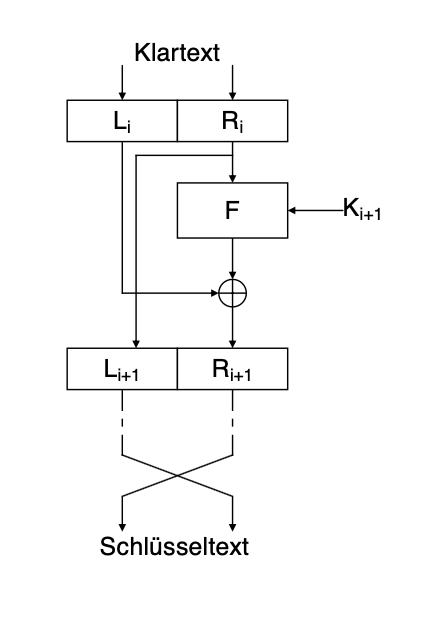
\includegraphics[width=.2\textwidth]{res/feistel.png}
  \caption{Feistel-Netzwerk}
  \label{fig:feistel}
\end{figure}
  \begin{enumerate}
    \item Berechnen Sie zwei Runden der Verschlüsselung und Entschlüsselung mit dem Feistel-Prinzip und den folgenden Werten:
      \begin{itemize}
        \item Klartext: 0011 0100
        \item Funktion F: binäres UND
        \item Rundenschlüssel K1: 1110
        \item Rundenschlüssel K2: 0001
      \end{itemize}
    \item Welche Eigenschaften sollte die Einwegfunktion F aufweisen, um mit ihrer Hilfe eine sichere Feistel-Chiffre zu erzeugen?
    \item Zeigen Sie, dass auch bei bei einer konstanten Einwegfunktion F sowohl die Ver- als auch die Entschlüsselung funktioniert.
    \item Benötigen Sie die Umkehrfunktion $F^{-1}$ von $F$, damit die Entschlüsselung klappt? Begründen Sie Ihre Antwort.
  \end{enumerate}

  \begin{solution}
    \begin{enumerate}
        \item
          \begin{itemize}
            \item Klartext: $(L_0, R_0) = 0011 \ 0100$
            \item Runde 1: $L_1 = R_0, \quad R_1 = L_0 \oplus R_0 \land K_1$
            \item Runde 2: $L_2 = R_1, \quad R_2 = L_1 \oplus R_1 \land K_2$
            \item Schlüsseltext: $(L_3, R_3) = (R_2, L_2) = 0101\ 0111$
          \end{itemize}

        \item Eigenschaften der Funktion $F$:
        \begin{itemize}
            \item Effizient berechenbar.
            \item Pseudozufällig, aber deterministisch.
            \item Nicht umkehrbar (Einhaltung der Sicherheit).
        \end{itemize}
        \item Eine konstante Funktion $F$ funktioniert, da die Struktur der Feistel-Chiffre die Umkehrbarkeit sicherstellt.
        \item Die Umkehrfunktion $F^{-1}$ ist nicht notwendig, da die Entschlüsselung über die symmetrische Struktur erfolgt.
    \end{enumerate}
  \end{solution}
\end{exercise}

\setcounter{subsection}{162}
\begin{exercise}{RSA: Eigenschaften und Sicherheit}\label{ex:rsa}
  Für die Erzeugung eines RSA-Schlüsselpaares wurde von Alice der Modulus $n= p \cdot q= 7 \cdot 17= 119$ gewählt.
  \begin{enumerate}
    \item Was muss für den öffentlichen Verschlüsselungsexponenten $c$, der gemeinsam mit dem Modulus $n$ veröffentlicht wird, gelten, damit dieser als Teil des RSA-Schlüssels verwendet werden kann?
    \item Warum kann eine mit RSA zu verschlüsselnde Nachricht $m$ nicht gleichzeitig einen Faktor $p$ und $q$ enthalten?
    \item Alice wählt den öffentlichen Verschlüsselungsexponenten $c= 5$. Berechnen Sie den zugehörigen geheimen Entschlüsselungsexponenten $d$ mithilfe des erweiterten euklidischen Algorithmus.
    \item Bei naiver Anwendung des RSA-Verfahrens wird eine Nachricht $m$, für die $1 < m < n$ gelten muss, ohne Veränderung mit dem öffentlichen Verschlüsselungsexponenten $c$ potenziert und modulo $n$ reduziert. Problematisch ist hierbei der multiplikative Homomorphismus des RSA-Verfahrens. Erläutern Sie kurz diese Eigenschaft anhand zweier Nachrichten $m_1$ und $m_2$.
    \item Wie könnte die Angreiferin Eve die Eigenschaft des multiplikativen Homomorphismus ausnutzen, um an die Klartextnachricht einer abgefangenen verschlüsselten Nachricht $s$, die an Alice adressiert war, zu gelangen? Zeigen Sie das Vorgehen anhand der abgefangenen verschlüsselten Nachricht $s= 101$, der eigens von Eve gewählten Zufallszahl $r= 22$ sowie dem multiplikativen Inversen der Zufallszahl $r^{-1} = 92 \mod 119$. Verwenden Sie auf Empfängerseite (Alice) den gegebenen RSA-Modulus, den öffentlichen Verschlüsselungsexponenten $c=11$ und den geheimen Entschlüsselungsexponenten $d=35$, der nur Alice, aber nicht Eve bekannt ist.
    \item Nennen Sie ein Anwendungsbeispiel, bei dem der multiplikative Homomorphismus des RSA-Verfahrens "ausgenutzt" bzw. gewollt angewendet wird.
  \end{enumerate}

  \begin{solution}
    \begin{enumerate}
        \item Der öffentliche Exponent $c$ muss teilerfremd zu $\varphi(n)$ sein, damit ein inverser Schlüssel existiert. Und zwischen 2 und $\varphi(n)$ liegen, um sicherzustellen, dass die Nachricht nicht trivial verschlüsselt wird.
        \item Da die Nachricht dann trivial verschlüsselt wäre mit $c = 0$, was auf $m=n$ schließen lässt.
        \item Berechnung des privaten Exponenten $d$ (mit $c = 5, n = 7 \cdot 17 = 119, \varphi(n) = 96$): $c \cdot d \equiv 1 \pmod{\varphi(n)}$
          \[ d = c^{-1} \mod \varphi(n) \implies d = 77 \]
        \item Angreifer können Produkte von Nachrichten entschlüsseln.
          \[ m_1 \cdot m_2 \mod n \implies c(m_1 \cdot m_2) = c(m_1) \cdot c(m_2) \]
        \item Eve berechnet $s'=s \cdot r^c \mod{n}$ und sendet $s'$ an Alice. Alice entschlüsselt $s'$ mit $s''=s'^d \mod{n}$ und erhält $s''=s \cdot r \mod{n}$. Durch Multiplikation mit $r^{-1}$ erhält Eve $s$.
        \item Ein Anwendungsbeispiel sind Berechnungen auf verschlüsselten Daten.
    \end{enumerate}
  \end{solution}
\end{exercise}

\setcounter{subsection}{1609}
\begin{exercise}{Würfeln mit RSA}
  Bob möchte Alice über das Internet das Ergebnis eines Würfelwurfs senden. Bob verschlüsselt das Ergebnis vor der Übertragung mit dem deterministischen RSA-Verfahren. Alice hat bereits ein RSA-Schlüsselpaar erzeugt und dabei die folgenden Parameter verwendet: $p_A = 5$, $q_A = 11$, $e_A = 3$, $d_A = 27$. Bob hat ebenfalls ein RSA-Schlüsselpaar erzeugt und dabei folgende Parameter verwendet: $p_B = 17$, $q_B = 5$, $e_B = 3$, $d_B = 43$. Die öffentlichen Schlüssel haben die beiden bereits über einen sicheren Kanal ausgetauscht.
  \begin{enumerate}
    \item Bob hat gewürfelt und möchte das Ergebnis nun an Alice senden. Er überträgt dazu $c_B = 9$. Zeigen Sie, dass eine passive Angreiferin (Eve), die lediglich die öffentlichen Schlüssel und $c_B$ kennt, mittels eines Chosen-Plaintext-Angriffs Bobs Wurfergebnis $m_B$ ermitteln kann. Welche Zahl hat Bob gewürfelt?
    \item Wie kann sich Bob vor diesem Angriff schützen?
  \end{enumerate}

  \begin{solution}
    \begin{enumerate}
        \item Da $m\in{1...6}$, probiert Eve alle möglichen Werte aus und verschlüsselt sie mit Bobs öffentlichem Schlüssel. Sie erhält $c_B = 9$ für $m_B = 4$. Bob hat also eine 4 gewürfelt.
        \item Bob kann sich schützen, indem er Zufallswerte oder Padding einfügt, um die deterministische Eigenschaft des RSA-Verfahrens zu verhindern.
    \end{enumerate}
  \end{solution}
\end{exercise}

\begin{exercise}{Forward Secrecy mit RSA}
  Zur Erreichung von Forward Secrecy wird häufig die Verwendung von symmetrischen Schlüsseln empfohlen, die regelmäßig gewechselt werden. Ein solcher Schlüsselaustausch kann beispielsweise mithilfe des Diffie-Hellman-Schlüsselaustauschs realisiert werden. Ein anderer Ansatz ist die Verwendung von asymmetrischen Schlüsseln, bei denen der private Schlüssel regelmäßig gewechselt wird. In dieser Aufgabe betrachten wir die Verwendung von RSA-Schlüsseln.
  \begin{enumerate}
    \item Erläutern Sie, wie Forward Secrecy mit RSA erreicht werden kann.
    \item Warum ist es problematisch, wenn ein Angreifer den privaten Entschlüsselungsexponenten eines RSA-Schlüssels erlangt?
    \item Wie kann ein Angreifer, der den privaten Entschlüsselungsexponenten eines RSA-Schlüssels erlangt hat, die Kommunikation zwischen zwei Parteien entschlüsseln, die Nachrichten mit diesem Schlüssel verschlüsselt haben?
    \item Wie kann Forward Secrecy mit RSA erreicht werden, wenn die Schlüssel regelmäßig gewechselt werden?
  \end{enumerate}

  \begin{solution}
    \begin{enumerate}
        \item Garnicht, RSA bietet keine Forward Secrecy.
        \item Da alle Nachrichten dann vom Angreifer entschlüsselt werden können.
        \item Angreifer entschlüsselt mittels Exponent
          \[ m=c^d \mod{n} \]
        \item Wenn die Schlüssel regelmäßig gewechselt werden, können bei Kompromittierung nur die Nachrichten entschlüsselt werden, die mit dem aktuellen Schlüssel verschlüsselt wurden.
    \end{enumerate}
  \end{solution}
\end{exercise}

\setcounter{subsection}{1615}
\begin{exercise}{Elliptische Kurven: EC-ElGamal}\label{ex:elliptic}
  Das ElGamal-Kryptosystem lässt sich auch auf elliptische Kurven übertragen. Dabei werden die Rechenoperationen mittels Punkten auf einer elliptischen Kurve vorgenommen. Betrachten Sie für die folgenden Teilaufgaben die elliptische Kurve $E(\text{GF}(p))$ mit der Form $y^2 \equiv x^3 + x + 6 \mod 11$.
  \begin{enumerate}
    \item Passen Sie die Operationen des ElGamal-Kryptosystems zur Schlüsselgenerierung, zur Entschlüsselung sowie zur Verschlüsselung an, sodass diese auf der Basis elliptischer Kurven operieren.
    \item Generieren Sie mithilfe Ihres Verfahrens aus Teilaufgabe a) ein geeignetes Schlüsselpaar auf der oben angegebenen elliptischen Kurve. Berechnen Sie dann die Verschlüsselung der Nachricht $m = (5, 2)$.
    \item Berechnen Sie die Entschlüsselung des Schlüsseltextes aus der vorherigen Teilaufgabe mit dem dort generierten geheimen Schlüssel.
    \item Zeigen Sie anschaulich, auf welcher Annahme die Sicherheit des Verfahrens beruht. Welcher Ausdruck müsste berechnet werden, damit Angreifende Schlüsseltexte ohne Kenntnis des geheimen Schlüssels leicht entschlüsseln könnten?
  \end{enumerate}

  \begin{solution}
    \begin{enumerate}
        \item 
          \begin{itemize}
            \item \textbf{Schlüsselgenerierung} mit Generaturpunkt $P$, privatem Schlüssel $d$ und öffentlichem Schlüssel $Q = d \cdot P$.
            \item \textbf{Verschlüsselung} von Nachricht $m$ mit Zufallswert $k$ und Schlüsseltext $(C_1, C_2) = (kP, m + kQ)$.
            \item \textbf{Entschlüsselung} des Schlüsseltextes $(C_1, C_2)$ mit privatem Schlüssel $d$ als $m = C_2 - d \cdot C_1$.
          \end{itemize}
        \item % TODO
        \item % TODO
        \item Die Sicherheit beruht darauf, dass es schwierig ist die Operation $Q=nP$ umzukehren.
    \end{enumerate}
  \end{solution}
\end{exercise}

\setcounter{subsection}{228}
\begin{exercise}{Verbindungsverschlüsselung in GSM}
  Welche Kommunikationsabschnitte sind in GSM verschlüsselt? Welche Kommunikationsabschnitte sind unverschlüsselt?

  \begin{solution}
    \begin{itemize}
        \item \textbf{Verschlüsselte Abschnitte}: Abschnitt zwischen Mobiltelefon und Basisstation.
        \item \textbf{Unverschlüsselte Abschnitte}: Basisstation $\to$ zentrale Netzwerkkomponenten (zB. MSC).
    \end{itemize}
  \end{solution}
\end{exercise}

\setcounter{subsection}{2226}
\begin{exercise}{Bluetooth-Authentifikation}
  Bei Bluetooth wird auf Basis der Funktion E22 die Authentifikation durchgeführt. Was sind die In- und Outputs der Authentifikation?

  \begin{solution}
    \begin{itemize}
        \item \textbf{Input:} Der Eingabewert der Funktion $ E22 $ ist ein gemeinsames Schlüsselpaar (Link Key), das während der Kopplung zwischen zwei Bluetooth-Geräten ausgetauscht wird.
        \item \textbf{Output:} Die Funktion erzeugt einen Authentication Code, der verwendet wird, um die Identität der Geräte gegenseitig zu authentifizieren.
    \end{itemize}
  \end{solution}
\end{exercise}

\setcounter{subsection}{2228}
\begin{exercise}{Mehrfachnutzung des IV in einem WEP-verschlüsselten WLAN}
  \begin{enumerate}
    \item Der in WEP verwendete Initialisierungsvektor (IV) ist 24 Bit groß und steht in einem Paket $P$ am Paketanfang vor dem Schlüsseltext. Wie viele Pakete können maximal erzeugt werden, wenn kein IV mehrfach verwendet werden soll? Wie sind die IVs von einem Teilnehmer des WLANs zu erzeugen, sodass eine Kollision möglichst spät auftritt? Welches Problem gibt es bei diesem Verfahren, wenn mehrere Teilnehmer kommunizieren?
    \item Nehmen Sie an, Sie haben die Pakete $P_1$ und $P_2$ empfangen:
    \begin{itemize}
      \item $P_1$: 00010 00111 11111 11110 11001 01001 00101 ...
      \item $P_2$: 00010 00111 11111 11110 11000 10011 00010 ...
    \end{itemize}
    Die ersten 10 Klartextbits des ersten Paketes $P_1$ lauten 10010 01100. Bestimmen Sie die ersten 10 Klartextbits des zweiten Paketes $P_2$.
  \end{enumerate}

  \begin{solution}
    \begin{enumerate}
        \item Maximal $ 2^{24} $ Pakete können erzeugt werden, da der IV 24 Bit groß ist. Um Kollisionen zu vermeiden, sollte der IV systematisch inkrementiert werden. Problematisch ist jedoch, dass bei mehreren Teilnehmern des WLANs die Wahrscheinlichkeit von IV-Kollisionen schnell steigt.
        \item Die ersten 10 Klartextbits des zweiten Pakets $ P_2 $ werden durch Vergleich mit $ P_1 $ berechnet:
        \[
        \texttt{Klartext}(P_2) = \texttt{Verschlüsselter\_Text}(P_2) \oplus \texttt{Schlüssel}(P_1).
        \]
        Nach Durchführung der XOR-Berechnung ergibt sich der Klartext.
    \end{enumerate}
  \end{solution}
\end{exercise}



\setcounter{section}{2023}
\section{Mock exam}

% \begin{exercise}{}
%  % TODO
%
%   \begin{solution}
%     % TODO
%   \end{solution}
% \end{exercise}



\setcounter{section}{2022}
\section{2nd exam}

\begin{exercise}{Betriebsarten}
  Betrachten Sie die Betriebsarten für Blockchiffren ECB, CBC und CTR.

  \begin{enumerate}
    \item Bei welchen Arten braucht man eine invertierbare Verschlüsselungsfunktion, bei welchen nicht? Begründen Sie.
    \item Bei welchen Arten lässt sich die Verschlüsselung parallelisieren?
    \item Im zweiten Block gibt es ein Bit mit einem additiven Fehler. Was kann noch entschlüsselt werden?
    \item Ein Bit fehlt im zweiten Block (nicht bekannt, wo das Bit fehlt). Was kann noch entschlüsselt werden?
    \item Ein ganzer Block fehlt. Was kann noch entschlüsselt werden?
    \item Zwei verschiedene Klartexte wurden mit CTR mit dem gleichen IV verschlüsselt. Zeigen Sie, dass ein Angreifer den zweiten Klartext entschlüsseln kann, wenn dieser den ersten Klartext und die beiden Schlüsseltexte hat.
  \end{enumerate}

  \begin{solution}
    \begin{enumerate}
        \item ECB und CBC benötigen invertierbare Verschlüsselungsfunktionen, da die Entschlüsselung der Chiffre notwendig ist. Der CTR beruht auf XOR-Verknüpfung der Klar- und Schlüsseltexte und Berechnung und Verschlüsselung der Zählerwerte sowohl beim Sender als auch beim Empfänger. Daher ist keine invertierbare Verschlüsselungsfunktion notwendig.
        \item Im ECB und CTR-Modus können die Blöcke parallel verschlüsselt werden, da sie unabhängig voneinander sind. Im CBC-Modus hängt die Verschlüsselung eines Blocks von der Verschlüsselung des vorherigen Blocks ab, daher ist keine Parallelisierung möglich.
        \item Bei allen Modi führt ein Bitfehler im zweiten Block dazu, dass dieser Block nicht entschlüsselt werden kann. Im CBC-Modus wird zusätzlich der Block 3 verändert, da die XOR-Verknüpfung mit dem vorherigen Block nicht mehr korrekt ist.
        \item Wenn die Blockgrenzen nicht bekannt sind, kann nur der erste Block entschlüsselt werden. Im CBC kann zusätzlich selbst bei bekannten Blockgrenzen nichts weiter entschlüsselt werden, da die XOR-Verknüpfung mit dem vorherigen Block nicht mehr korrekt ist.
        \item Bei ECB und CTR können alle anderen Blöcke korrekt entschlüsselt werden, da sie unabhängig voneinander sind. Im CBC-Modus kann kein nachfolgender Block entschlüsselt werden, da die XOR-Verknüpfung mit dem vorherigen Block nicht mehr korrekt ist.
        \item Da $m_1$ und $c_1$ kann daraus der Pseudozufallszahlenstrom $s=c_1\oplus m_1$ berechnet werden. Hiermit lässt sich dann $m_2=c_2\oplus s$ berechnen.
    \end{enumerate}
  \end{solution}
\end{exercise}

\begin{exercise}{Elliptische Kurven}
  \begin{enumerate}
    \item Auf welcher mathematischen Schwierigkeit basiert der ECC?
    \item Berechnen Sie die Punkte auf der folgenden elliptischen Kurve: $a = 6$, $b = 1$, $p = 11$ (allgemeine Formel war gegeben).
    \item Nennen Sie zwei Vorteile, die ECC gegenüber sicherheitsmäßig vergleichbaren Verfahren hat.
  \end{enumerate}

  \begin{solution}
    \begin{enumerate}
        \item ECDLP (Elliptic Curve Discrete Logarithm Problem): Das Problem besteht darin, die Operation $Q=nP$, welche mathematisch einfach zu berechnen ist, umzukehren.
        \item Punkte auf der elliptischen Kurve $y^2 = x^3 + 6x + 1 \pmod{11}$:
          \[ \{(2,4), (4,5), (4,6), (6,3), (6,8), (7,5), (7,6), (8,2), (8,9), (9,4), (9,7), (10,1), (10,10)\} \]
        \item Vorteile von ECC:
          \begin{itemize}
              \item Kürzere Schlüssel bei gleicher Sicherheit (z. B. ECC-256 entspricht RSA-3072).
              \item Geringere Speicher- und Rechenanforderungen.
          \end{itemize}
    \end{enumerate}
  \end{solution}
\end{exercise}

\begin{exercise}{Zertifikate}
  Das Zertifizierungsmodell ist transitiv anzunehmen.

  \begin{figure}
  \centering
  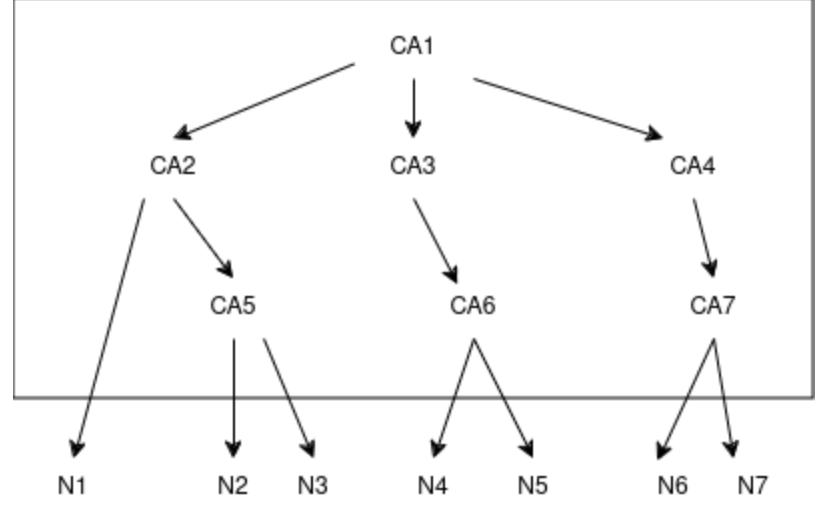
\includegraphics[width=.6\textwidth]{res/2023-1.png}
  \caption{Transitive Zertifizierung}
  \label{fig:zertifizierung}
\end{figure}

  \begin{enumerate}
    \item Erklären und grenzen Sie die Begriffe Signatur und Zertifikat voneinander ab.
    \item N7 möchte N3 eine Nachricht schicken. Welchen CAs muss N7 vertrauen?
    \item N7 möchte zusätzlich N5 eine Nachricht schicken. Welchen CAs muss N7 vertrauen, so dass die Anzahl an CAs minimal ist?
    \item CA2 fällt aus. Wie können wir die Kommunikation aus b) trotzdem realisieren (Was \& Wie)? Was können wir für N1 tun?
    \item Trust on First Use: Keine CAs, Schlüssel wird bei erster Kommunikation an Kommunikationspartner geschickt, sobald und bei späteren Kommunikationen überprüft. Wenn Kommunikation und es gibt schon anderen Schlüssel, deny. Nennen und erklären Sie zwei Vorteile und zwei Nachteile.
  \end{enumerate}

  \begin{solution}
    \begin{enumerate}
        \item Eine Signatur dient der Authentifizierung und Integritätsprüfung einer Nachricht. Ein Zertifikat enthält den öffentlichen Schlüssel eines Teilnehmers sowie die Signatur einer vertrauenswürdigen Zertifizierungsstelle (CA), die die Authentizität des Schlüssels bestätigt.
        \item N7 muss den CAs vertrauen, die die Zertifikate von N3 und allen relevanten Zwischenstellen signiert haben.
        \item N7 muss nur den CAs vertrauen, die sowohl N3 als auch N5 direkt oder indirekt zertifizieren. Dies minimiert die Anzahl der erforderlichen CAs.
        \item Wenn CA2 ausfällt, können alternative Zertifikate verwendet werden, die von anderen vertrauenswürdigen CAs ausgestellt wurden. Ein neuer Vertrauenspfad kann erstellt werden.
        \item Vorteile von Trust on First Use (TOFU):
          \begin{itemize}
              \item[+] Kein zentraler CA-Betrieb notwendig.
              \item[+] Schlüssel können einfach ausgetauscht werden.
              \item[-] Unsicherheit beim ersten Austausch.
              \item[-] Bei Schlüsseländerungen kann es zu Problemen kommen.
          \end{itemize}
    \end{enumerate}
  \end{solution}
\end{exercise}

\begin{exercise}{Forward Secrecy mit RSA}
  Zur Erreichung von Forward Secrecy erzeugt Alice auf ihrem Server mit dem RSA-Verfahren einen privaten Schlüssel $d$ sowie den dazu passenden öffentlichen Schlüssel $c$, den sie persönlich an ihre Nutzerinnen und Nutzer verteilt. Zusätzlich erzeugt der Server von Alice bei jedem Verbindungsaufbau ein neues kurzlebiges (engl. ephemeral) RSA-Schlüsselpaar, das aus einem öffentlichen Schlüssel $c_e$ und einem geheimen Schlüssel $d_e$ besteht. Der Server signiert mit dem privaten Schlüssel $d$ den neuen öffentlichen Schlüssel $c_e$ und sendet diesen zusammen mit der Signatur über die aufgebaute Verbindung an die Kundin. Die Kundin prüft anschließend die Signatur mithilfe des zuvor von Alice erhaltenen öffentlichen Schlüssels $c$. Ist die Signatur korrekt, nutzt die Kundin $c_e$, um einen neuen, zufällig generierten symmetrischen AES-Schlüssel $k$ zu verschlüsseln. Die weitere Kommunikation in dieser Verbindung wird symmetrisch mit $k$ verschlüsselt. Nach Verbindungsende löscht Alices Server $d_e$, $c_e$ und $k$.

  \begin{enumerate}
    \item Welche Verbindungen könnten von einem sehr starken Angreifer wie einem Nachrichtendienst noch entschlüsselt werden, wenn dieser Zugriff auf den Server bekommt? Begründen Sie Ihre Antwort.
    \item Skizzieren Sie einen Angriff, der möglich wäre, wenn die Kundin die Signatur nicht prüft. Erläutern Sie die einzelnen nötigen Schritte.
    \item Alice ist das Verfahren zu langsam. Sie nimmt nun folgende Änderung vor: Statt jedes Mal bei der Erzeugung von $c_e$ und $d_e$ neue Primzahlen $p$ und $q$ für den Modulus $N_e$ zu generieren, verwendet sie immer die gleichen Primzahlen. Nun wählt sie lediglich den öffentlichen Exponenten $c_e$ neu und berechnet einen dazugehörigen geheimen Exponenten $d_e$. Warum ist dies keine gute Idee? Zeigen Sie, wie sich dieses geänderte Verfahren angreifen lässt, um aufgezeichnete Verbindungen zu entschlüsseln.
  \end{enumerate}

  \begin{solution}
    % TODO
  \end{solution}
\end{exercise}



\setcounter{section}{2021}
\section{1st exam}

\begin{exercise}{Kryptographie}
 \begin{enumerate}
  \item Erläutern Sie zwei Ursachen, die dafür sorgen, dass fast alle kryptographischen Algorithmen mit der Zeit nicht mehr Standard sind.
  \item Sie möchten einen Text so verschlüsseln, dass er auch in 98 Jahren nicht ohne Kenntnis des von Ihnen versteckten Schlüssels entschlüsselt werden kann. Welches Verfahren wählen Sie dazu? Begründen Sie Ihre Entscheidung. Warum wird das Verfahren heutzutage nicht überall benutzt?
  \item Gegeben eine Chiffre, welche Buchstaben A-N mit Buchstaben N-Z vertauscht. Und gleichzeitig muss die Länge der Nachricht immer gleich sein. Bewerten Sie die Sicherheit der Chiffre und die beiden Eigenschaften (Polyalphabetische Verschlüsselung nur mit Vertauschen und die gleiche Länge der Nachricht).
 \end{enumerate}

 \begin{solution}
  \begin{enumerate}
      \item Gründe für den Wechsel kryptographischer Algorithmen:
      \begin{itemize}
          \item **Technologischer Fortschritt:** Schnellere Computer ermöglichen effizientere Brute-Force-Angriffe.
          \item **Neue Angriffe:** Fortschritte in der Kryptoanalyse decken Schwachstellen auf, wie z. B. Differential- oder lineare Kryptoanalyse.
      \end{itemize}
      \item Das **One-Time-Pad** bietet absolute Sicherheit und bleibt auch nach 98 Jahren sicher. Es wird nicht flächendeckend eingesetzt, da:
      \begin{itemize}
          \item Der Schlüssel so lang wie der Klartext sein muss.
          \item Der sichere Schlüsselaustausch und die Speicherung unpraktisch sind.
      \end{itemize}
      \item Die Chiffre, die Buchstaben $ A-N $ mit $ N-Z $ vertauscht, ist nicht sicher:
      \begin{itemize}
          \item **Polyalphabetische Verschlüsselung:** Nicht erfüllt, da nur ein Alphabet genutzt wird.
          \item **Länge bleibt gleich:** Diese Eigenschaft bewahrt Muster im Schlüsseltext, was statistische Angriffe erleichtert.
      \end{itemize}
  \end{enumerate}
\end{solution}
\end{exercise}

\begin{exercise}{Elliptische Kurven}
  \begin{enumerate}
    \item Berechnen Sie für die folgenden Parameter alle Punkte auf der Kurve: $a = 2$, $b = 3$, $p = 7$.
    \item Elgamal mit elliptischen Kurven wurde vorgestellt. Zeigen Sie, warum dieses Verfahren mit beliebigen Parametern funktioniert.
    \item Vergleichen Sie den Elgamal aus der Vorlesung mit dem gegebenen. Auf welchem Prinzip beruht die Sicherheit? Denken Sie, dass er sicherer ist? Warum?
  \end{enumerate}

  \begin{solution}
    \begin{enumerate}
        \item Punkte auf der elliptischen Kurve $ y^2 = x^3 + 2x + 3 \mod 7 $:
        \[
        \{(1, 1), (2, 2), (4, 5), (6, 3)\}.
        \]
        \item Das ElGamal-Verfahren mit elliptischen Kurven funktioniert, weil die Addition von Punkten und die Multiplikation mit einem Skalar die Gruppenstruktur der Kurve erhalten. Dadurch bleibt das diskrete Logarithmusproblem schwer lösbar.
        \item Vergleich:
        \begin{itemize}
            \item Beide basieren auf dem diskreten Logarithmusproblem.
            \item ECC-ElGamal ist effizienter, da kürzere Schlüssel benötigt werden.
        \end{itemize}
    \end{enumerate}
  \end{solution}
\end{exercise}

\begin{exercise}{Zertifikate}
  \begin{enumerate}
    \item Es wurden 3 verschiedene Möglichkeiten gegeben, einen Schlüssel von verschiedenen Schlüsselpartnern (S, V, C, T) zu kombinieren. Alle Teilschlüssel werden aneinander gehängt l/4. 3 der Teilschlüssel wird aneinander gehängt und der letzte Teilnehmer bestimmt die Reihenfolge. Alle Schlüssel werden XOR berechnet. Bewerten Sie die Sicherheit der Verfahren.
    \item Gegeben ist ein Zertifikatsbaum mit 5 Teilnehmern. $E \rightarrow D$, $E \rightarrow B$, $E \rightarrow A$, $E \rightarrow C$, $C \rightarrow B$, $A \rightarrow B$, $G \rightarrow \emptyset$. Betrachten Sie die Zertifizierungsrelation. $G$ möchte jetzt zusätzlich eine verschlüsselte Nachricht an $B$ senden. Welcher Zertifizierungsstelle bzw. welchen Zertifizierungsstellen muss $G$ mindestens vertrauen, um das Zertifikat von $B$ prüfen zu können?
    \item Wählen Sie Ihre Lösung so, dass die Anzahl an Zertifizierungsstellen, denen $N4$ (explizit) vertrauen muss, minimal ist.
    \item In der Zertifizierungsrelation aus Teilaufgabe c) wird die Zertifizierungsstelle $C$ kompromittiert und fällt deshalb aus. $G$ möchte eine verschlüsselte Nachricht an $C$ senden. Welche Maßnahme ermöglicht es $G$, das Zertifikat von $B$ trotz des Ausfalls von $CA4$ zu überprüfen?
  \end{enumerate}

  \begin{solution}
    \begin{enumerate}
        \item Sicherheitsbewertung der Verfahren:
        \begin{itemize}
            \item **Alle Teilschlüssel aneinanderhängen:** Angreifbar durch Brute-Force-Angriffe.
            \item **Drei Teilschlüssel aneinanderhängen:** Sicherheitsgewinn gegenüber der ersten Methode.
            \item **XOR aller Schlüssel:** Höchste Sicherheit, solange alle Schlüssel zufällig und unabhängig sind.
        \end{itemize}
        \item Zertifikatsbaum: N7 vertraut CAs, die N3 und $ B $ direkt zertifizieren.
        \item Minimale Anzahl an CAs: Es reicht aus, der CA zu vertrauen, die die Zertifikate für $ B $ und $ N3 $ signiert hat.
        \item Maßnahme bei Kompromittierung: Alternativer Zertifizierungsweg über eine andere CA. Neue Zertifikate können erstellt werden, um Vertrauen zu erhalten.
    \end{enumerate}
  \end{solution}
\end{exercise}

\begin{exercise}{GSM}
  \begin{enumerate}
    \item Sagen Sie zu folgenden Abkürzungen welche Funktion sie im GSM erfüllen: $Ki$, $IMSI$, $RAND$, $SRES$, $LAI$, $MSISDN$, $Kc$.
    \item Welche dieser Abkürzungen ist auch noch im UMTS enthalten bzw. mit ähnlicher Funktion aber anderen Namen?
  \end{enumerate}

  \begin{solution}
    \begin{enumerate}
        \item Abkürzungen im GSM und ihre Funktion:
        \begin{itemize}
            \item $ K_i $: Geheimer Schlüssel zur Authentifizierung und Verschlüsselung.
            \item $ IMSI $: Einzigartige Kennung des Mobilfunkteilnehmers.
            \item $ RAND $: Zufällige Herausforderung zur Authentifizierung.
            \item $ SRES $: Antwort des Mobilgeräts auf $ RAND $, basierend auf $ K_i $.
            \item $ LAI $: Standortkennung für Mobilitätsmanagement.
            \item $ MSISDN $: Telefonnummer des Teilnehmers.
            \item $ K_c $: Schlüssel zur Verschlüsselung des Datenverkehrs.
        \end{itemize}
        \item Diese Funktionen sind auch im UMTS enthalten, jedoch oft mit verbesserten Sicherheitsmechanismen (z. B. längere Schlüssel, stärkere Algorithmen).
    \end{enumerate}
  \end{solution}
\end{exercise}

\end{document}